\section{Experimentació}

\subsection{Se\lgem ecció dels operadors}
Per a realitzar l'experiment 1 ha fixat en nombre d'usuaris a 200 i el nombre de conductors a 100.
Posteriorment s'ha executat 10 cops amb cada un dels conjunts d'operadors.


Els resultats son:
        El conjunt d'operadors 1 produeix millor resultat que el conjunt 2.
        Suposam que aixo es degut a que l'operador genera mes estats per a cada iteració.

        No hi ha diferencia significativa en el temps d'execució amb els dos conjunts d'operadors (comprovar).
        Suposam que aquest resultat es degut a que, encara que el conjunt d'operadors 2 genera menys estats
        que el conjunt 1, les operacions son mes costoses.



        (TAULA AMB ELS RESULTATS)

\subsection{Se\lgem ecció de la generació de l'estat inicial}
per arealitzar l'experiment 2 s'ha fixat el nombre d'usuaris i el nombre de conductors com a lanterior experiment.                                                                                   
S'ha executat 10 cops amb cada estrategia de generació inicial.
                                                                                                                                                                                                     
Els resultats son:                                                                                                                                                                                   
        La estrategia de generació inicial (Repartir tots els conductors) produeix millors resultats.
                                                                                                                                                                                                     
        No existeix diferencia en el cost temporal de generacio de les solucions inicials, ja que                                                                                                    
        ambdues estrategies son molt simples asimptoticament theta(n)                                                                                                                                
                                                                                                                                                                                                     


        (TAULA AMB ELS RESULTATS)



\subsection{Se\lgem ecció dels paràmetres del Simulated Anealing}
Per a determinar els paràmetres que obtenen un millor resultat per a l'execució de l'algorisme \emph{simulated annealing},
hem executat reiterades vegades, aproximadament 10, l'algorisme amb diferents parametres per a \texttt{lambda} i \texttt{k}, concretament s'ha fet amb
\texttt{[0.1,0.01,0.001,0.0001]} i \texttt{[1,5,25,125]} repectivament, fixant el nombre d'iteracions en 2000.

El millor resultat s'ha obtingut amb els parametres k = 5 i lambda = 0.01, com indica el seguent grafic (fig. \ref{test3-gr1}).

\begin{figure}[H]
\begin{center} 
 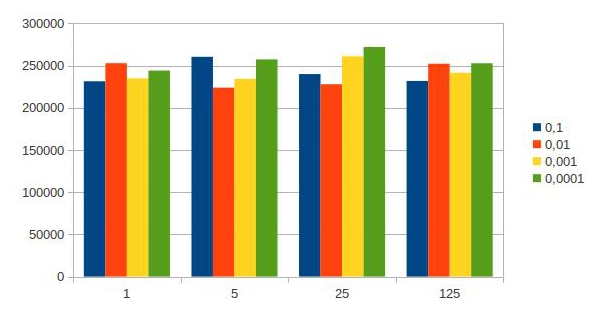
\includegraphics[width=0.6\textwidth]{figures/test3-gr1.jpg}
\label{test3-gr1}
\end{center}
\end{figure}

Fixats aquests dos paràmetres en els valors que han obtingut millor resultat, s'ha ajustat el nombre d'iteracions executant diverses 
vegades l'algorisme amb un nombre diferent d'iteracions. Es pot veure (fig. \ref{test3-gr2}) en el seguent gràfic el millor valor per al nombre d'iteracions.

\begin{figure}[H]
\begin{center}
 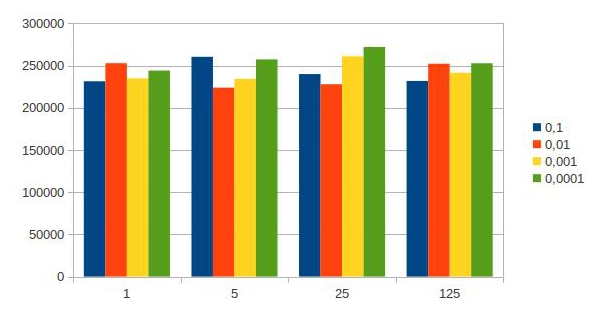
\includegraphics[width=0.6\textwidth]{figures/test3-gr1.jpg}
 \label{test3-gr2}
\end{center}
\end{figure}



Aleshores, podem comparar els resultats obtinguts amb simulated Annealing i Hill climbing.

Es pot observar (fig. \ref{test3-gr3} i \ref{test3-gr4}) que el Simulated Annealing obte millors resultats que el Hill Climbing. Per contra, te un temps d'execució molt mes elevat.

\begin{figure}[H]
\begin{center} 
 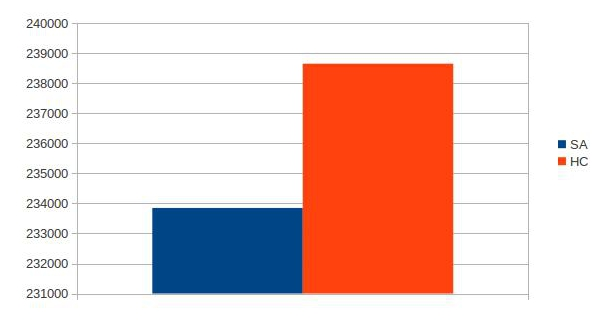
\includegraphics[width=0.6\textwidth]{figures/test3-gr3.jpg}
\label{test3-gr3}
\end{center}
\end{figure}


\begin{figure}[H]
\begin{center}
 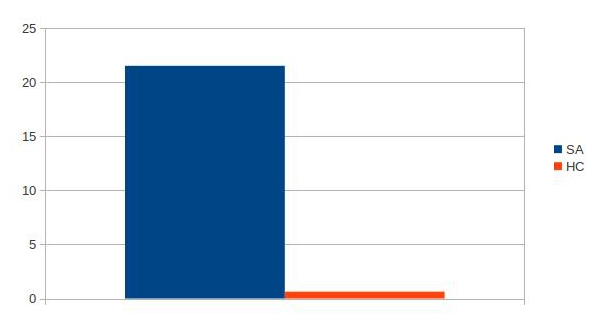
\includegraphics[width=0.6\textwidth]{figures/test3-gr4.jpg}
 \label{test3-gr4}
\end{center}
\end{figure}


\subsection{Observació de l'evolució temporal del Hill Climbing}

\subsection{Se\lgem ecció dels valors de ponderació del segon heurístic}

\subsection{Se\lgem ecció del valor de \emph{M} per millor inicialització del problema}